\begin{table*}[h]\centering
\begin{tabular}{|l|c|c|c|c|c|}
\hline
                            & PQL2 & PQL3 & PQL+ & WQSP & CWQ \\
\hline
KV-MemNN \cite{DBLP:conf/emnlp/MillerFDKBW16}    & 72.2 & 67.4 & -    & 46.7 / - & 21.1\footnote{The original paper only reports scores on development set.} / -      \\
IRN \cite{DBLP:conf/coling/ZhouHZ18}                         & 72.5 & 71.0   & 52.9 & -    & -         \\
HR-BiLSTM \cite{DBLP:conf/acl/YuYHSXZ17}                  & 97.5 & 87.9 & 92.9 & 62.9 / 62.3 & 33.3 / 31.2         \\
ABWIM \cite{DBLP:journals/corr/abs-1801-09893}                      & 94.3 & 89.3 & 92.6 & -    & -         \\
UHop\footnote{We use the best reported setup from the original paper, aka. ABWIM with UHop.} \cite{DBLP:conf/naacl/ChenCCNK19}                       & 97.5 & 89.3 & 92.3 & -    & -         \\
GRAFT-Net \cite{DBLP:conf/emnlp/SunDZMSC18}                  & -    & -    & -    & 67.8 / 62.5 & 30.1 / 26.0      \\
KBQA with Topic Units \cite{DBLP:conf/ijcai/LanW019}                  & -    & -    & -    & 68.2 / 67.9 & 39.3 / 36.5      \\
\hline
Our Method-obj1             & 98.3 & 97.1 & 97.5 &    62.8 / 62.3  &           \\
Our Method-obj2             &   -   &   -   &   -   &  65.4 / 65.1     &           \\
Our Method-obj3             &     - &  -    &   -   &   67.9 / 67.0    &           \\
Our Method-obj3+new\_decode & -     &   -   &    -   &     &          \\
\hline
\end{tabular}
\caption{\fontsize{10}{12}\selectfont We report Accuracy on PQL and hits@1 and F1 on WQSP and CWQ. All scores except our method are copied from the previous published papers. obj1/2: $P(ans, path|x)= P(ans|path,x)*P(path|x)$ with single/multiple reasoning paths for one sample. obj3: $P(ans) = sum_path(P(ans|path,x)*P(path|x))$, new\_decode: use beam search and multi paths in decoding.}\label{tab:main}
\end{table*}


\begin{figure}[h]
\centering
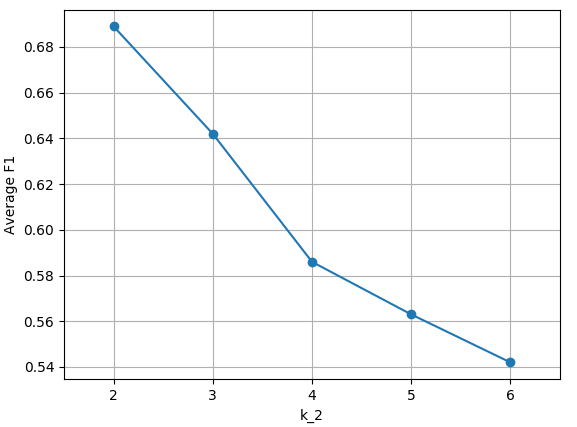
\includegraphics[width=0.85\columnwidth]{figs/fig2.png}
\vspace{-2ex}
\caption{\fontsize{10}{12}\selectfont Average F1 over different thresholds on \textsc{WebQuestionSp} dataset.}
\label{fig:k2}
\end{figure}


\begin{table}[h]\centering
\resizebox{1.01\columnwidth}{!}{
\begin{tabular}{|l|c|c|}
\hline
                           & WQSP & CWQ \\
\hline
%KV-MemNN \cite{DBLP:conf/emnlp/MillerFDKBW16}    & 46.7 / - & 21.1\tablefootnote{The original paper only reports scores on development set.} / -      \\
HR-BiLSTM \cite{DBLP:conf/acl/YuYHSXZ17}                  & 62.9 / 62.3 & 33.3 / 31.2         \\
GRAFT-Net \cite{DBLP:conf/emnlp/SunDZMSC18}                & 67.8 / 62.5 & 30.1 / 26.0      \\
KBQA-GST \cite{DBLP:conf/ijcai/LanW019}          & 68.2 / 67.9 & 39.3 / \textbf{36.5}      \\
\hline
Our Method-joint\_prob             &    62.8 / 62.3  &   36.7 / 31.4        \\
Our Method-joint\_prob\_multiple\_paths             &  65.4 / 65.1     &    - / -       \\
Our Method-marginal\_prob\_with\_true\_label             &   \textbf{68.9} / \textbf{68.5}    &      \textbf{39.4} / 34.8     \\
Our Method-marginal\_prob\_without\_true\_label             &   68.8 / 68.3    &       33.0 / 27.6    \\
%Our Method-obj3+new\_decode  &     &          \\
\hline
\end{tabular}
}
\caption{\fontsize{10}{12}\selectfont We report hits@1 / F1 on WQSP and CWQ.}\label{tab:wqsp_cwq}
\end{table}